\documentclass[a4paper,12pt,twoside,openany]{report}

\usepackage[utf8]{inputenc}
\usepackage[OT4]{fontenc}
\usepackage{polski}
\usepackage{multirow}
\usepackage{graphicx}
\graphicspath{ {./images/} }
\usepackage[nottoc]{tocbibind}
\usepackage{url}
\usepackage{subcaption}
\usepackage{float}

\newcommand{\specialcell}[2][c]{%
  \begin{tabular}[#1]{@{}c@{}}#2\end{tabular}}

\linespread{1.5} 


\begin{document}
\begin{titlepage}
    \begin{center}
        \large
        \textbf{Politechnika Poznańska}\\
        Wydział Informatyki i Telekomunikacji\\
        Instytut Informatyki\\
        \vspace{1.5cm}
            
        \textbf{Dominik Krystkowiak}\\
        Praca dyplomowa magisterska\\
        
        \vspace{1cm}
        \Huge
        \textbf{
        Analiza i zastosowanie zaawansowanych mechanizmów rekomendacji}
            
        \vfill
        \begin{flushright}\large
        Promotor dr inż. Anna Grocholewska-Czuryło\end{flushright}
        \vspace{0.8cm}
            
        \large
        2020
            
    \end{center}
\end{titlepage}

\thispagestyle{empty}\vspace*{\fill}%
\begin{center}KARTA DYPLOMOWA\end{center}%
\vfill\cleardoublepage%

\thispagestyle{plain}
\begin{center}
    \textbf{Abstract}
\end{center}
Lorem ipsum dolor...

\tableofcontents* 
\cleardoublepage%


\chapter{Wstęp}

\indent Rekomendacja (zgodnie z jedną z definicji zawartej w słowniku języka polskiego) oznacza “pozytywną opinię wydaną o kimś” \cite{pwn}. Każdy z nas w swoim życiu spotkał się z poleceniem przez znajomego ostatnio przeczytanej książki lub obejrzanego filmu. Na tej podstawie można wywnioskować, że pierwsze mechanizmy rekomendacji powstały na długo przed rozpowszechnieniem handlu internetowego, gdzie aktualnie zyskują coraz większą popularność.

\indent W dobie ciągłego postępu oraz globalizacji systemy rekomendacyjne wchodzące w skład złożonych serwisów odgrywają coraz większą rolę. Wcześniej stosowane sposoby prezentacji (takie jak reklama czy newslettery) produktu stały się dla użytkowników zbyt natarczywe lub nie przynosiły firmom oczekiwanego rezultatu. Stąd korporacje i przedsiębiorstwa inwestują coraz większe pieniądze w implementację i wdrożenie systemów rekomendacyjnych.

\indent Głównym elementem pracy jest dokonanie przeglądu mechanizmów rekomendacji, podział ze względu na zastosowanie oraz opracowanie bezpiecznego protokołu oraz porównanie jego wydajności i skuteczności.

\indent Pierwszy rozdział przedstawia ogólną charakterystykę systemów rekomendacyjnych, ich cechy charakterystyczne oraz założenia. Ponadto przedstawiono najczęściej stosowane oraz sprawdzone komercyjnie rozwiązania podczas implementacji tego typu oprogramowania. Także omówiono problemy oraz wyzwania z którymi muszą zmagać się programiści tworząc nowoczesne systemy rekomendacyjne.  

\indent W kolejnym rozdziale został przedstawiony problem związany z bezpieczeństwem danych użytkownika oraz możliwością jego identyfikacji po wystawionych ocenach.

\indent W dalszej części pracy pokazano możliwe rozwiązanie problemu związanego z identyfikacją użytkownika.
W podsumowaniu omówiono otrzymane wyniki oraz możliwości udoskonalenia mechanizmu bezpieczeństwa 

\chapter{Przegląd systemów rekomendacyjnych}

Systemy rekomendacyjne pomagają użytkownikom w zdobyciu wartościowych i spersonalizowanych informacji z dużego źródła danych. Większość przypadków działania takiego systemu opiera się na przewidzeniu preferencji użytkownika na podstawie wcześniej zgromadzonych danych.

Ważnym momentem w historii systemów rekomendacyjnych był otwarty konkurs \textit{Netflix Prize} polegający na zaproponowaniu najlepszego algorytmu \textit{collaborative filtering} mającego na celu przewidzenie ocen użytkowników dla filmów, opierając się wyłącznie na poprzednich ocenach, bez dodatkowych informacjach o użytkownikach i filmach. W tym celu opublikowano zbiór testowy zawierający ponad 100 milionów ocen wystawionych przez 500 tysięcy anonimowych użytkowników. W wyzwaniu wzięło udział ponad 48 tysięcy zespołów z 182 państw \cite{netflix_prize}.

Po konkursie \textit{Netflix Prize} głównym motywem przewodnim w pracach naukowych stała się faktoryzacja macierzy. Również w celu zwiększenia skuteczności algorytmu uwagę poświęcono takim zagadnieniom jak: wykorzystanie sieci społecznościowych oraz uczenia głębokiego w systemach rekomendacyjnych \cite{recent_developments}.

Rozdział omawia sposób działania systemów rekomendacyjnych, główne problemy i wyzwania stawiane tym systemom. Także przedstawiono popularne mechanizmy, sposoby ewaluacji oraz główne zalety poszczególnych rozwiązań.

\section{Założenia systemów rekomendacyjnych}

Głównymi zadaniami systemów rekomendacyjnych jest odfiltrowanie przedmiotów (na przykład: filmy, książki), które są dla użytkownika potencjalnie mało interesujące lub nieatrakcyjne. Użytkownik korzystający z serwisu wspieranego przez tego typu systemy otrzymuje jako proponowane, mały, spersonalizowany zestaw produktów z całego zbioru.

Systemy rekomendacyjne mogą zostać podzielone na dwie grupy ze względu na podejście \cite{recent_developments}: spersonalizowane oraz niespersonalizowane. Pierwsze opierają swoje działanie na zebranych danych użytkownika. Informacje o odwiedzających mogą zostać zdobyte poprzez monitorowanie zachowań użytkowników lub poprzez bezpośrednie zapytanie użytkowników o ich preferencje. Natomiast podejście niespersonalizowane bazuje na zachowaniach pozostałych użytkowników.

Dane zazwyczaj przedstawiane są w formie dwuwymiarowej macierzy $R = U \times I$, gdzie U jest to zbiór n użytkowników oraz I zbiór m przedmiotów. Tabela \ref{macierzUI} przedstawia przykład takiej macierzy, wiersze reprezentują użytkowników, kolumny przedmioty, oceny są w przedziale 1 do 5, natomiast 0 oznacza brak oceny. Aby uzyskać lepsze rekomendacje systemy mogą wykorzystać macierze o większej liczbie wymiarów (zawierających czas, lokalizację czy informacje uzyskane z mediów społecznościowych).

Dzięki coraz lepszym technikom zdobywania danych oraz spadającej tendencji do udzielania ocen wśród klientów, popularnym stało się wykorzystanie domniemanych danych (\textit{ang. implict data}) takich jak: liczba kliknięć lub wyświetleń do budowania akademickich oraz branżowych systemów rekomendacyjnych \cite{Adomavicius2005}. Dane takie w przeciwieństwie do informacji sprecyzowanych (\textit{ang. explict data}) nie opierają się o negatywne sprzężenie zwrotne oraz nie wymagają metryki pewności (nawiązują do częstotliwości występowania zjawiska).

\label{macierzUI}
\begin{table}[h]
\centering
\caption{Przykład macierzy użytkownik-przedmiot.}
\begin{tabular}{|c|c|c|c|c|c|}
\hline
&
Przedmiot1 &
Przedmiot2 &
Przedmiot3 &
Przedmiot4 &
Przedmiot5
\\
\hline
  
Użytkownik1 &
1 &
5 &
4 &
2 &
3
\\
\hline
  
Użytkownik2 &
5 &
0 &
2 &
4 &
0
\\
\hline

Użytkownik3 &
1 &
0 &
4 &
0 &
4
\\
\hline

Użytkownik4 &
3 &
0 &
3 &
1 &
5
\\
  \hline

Użytkownik5 &
2 &
0 &
2 &
0 &
3
\\
\hline
\end{tabular} 
\end{table}

Ze względu na rodzaj wyjścia (otrzymanego wyniku) systemy rekomendacyjne możemy podzielić na następujące dwie grupy: pojedyncza predykcja oraz top-N predykcji. Pierwsza polega na przewidzeniu dokładnej oceny, którą użytkownik mógłby dać przedmiotowi, natomiast drugie podejście zwraca N nieocenionych przedmiotów, które mogłyby najbardziej przypaść do gustu użytkownikowi.


\section{Problemy i wyzwania}
Nowoczesne systemy oparte o rekomendacje muszą radzić sobie z wieloma trudnościami. Problemy dotyczą zarówno małej liczby danych jak i zachowaniem grupy lub pojedynczych użytkowników. Poniżej przedstawiono najczęstsze wyzwania stawiane przed systemami rekomendacyjnymi. \cite{trendsProblems}

Rzadkość danych - następuje w momencie, gdy wielu użytkowników oceniło tylko kilka przedmiotów przez co system rekomendacyjny nie może poznać preferencji użytkownika (macierz użytkownik-przedmiot ma zbyt wiele pustych wartości). 

\label{macierzRzadkosc}
\begin{table}[h]
\centering
\caption{Przykład rzadkości danych w macierzy.}
\begin{tabular}{|c|c|c|c|c|c|}
\hline
&
Przedmiot1 &
Przedmiot2 &
Przedmiot3 &
Przedmiot4 &
Przedmiot5
\\
\hline
  
Użytkownik1 &
NaN &
NaN &
NaN &
NaN &
3
\\
\hline
  
Użytkownik2 &
NaN &
NaN &
NaN &
4 &
NaN
\\
\hline

Użytkownik3 &
1 &
NaN &
NaN &
NaN &
NaN
\\
\hline

Użytkownik4 &
3 &
NaN &
3 &
NaN &
5
\\
  \hline

Użytkownik5 &
NaN &
NaN &
2 &
NaN &
NaN
\\
\hline
\end{tabular} 
\end{table}

Skalowalność - systemy rekomendacyjne wraz ze wzrostem liczby użytkowników muszą radzić sobie z napływem coraz większej liczby danych do przetworzenia. Gdy takie dane wynoszą miliony użycie standardowych mechanizmów rekomendacyjnych może powodować otrzymanie wyników rekomendacji z dużym opóźnieniem (niewystarczający krótki czas na uzyskanie odpowiedzi). Bardziej złożony system wymaga większej liczby osób usprawniających oraz zarządzających jego działaniem, co równa się większemu kosztowi utrzymania zarówno pracowników jak i sprzętu komputerowego na którym taki system jest wdrożony.
    
Czarna owca - zjawisko występuje w momencie, gdy preferencje jednego z użytkowników nie pokrywają się z wyodrębnionymi grupami użytkowników, stąd użytkownik nie będzie w stanie otrzymać spersonalizowanych rekomendacji (przykład przedstawiony na rys. \ref{fig:grey-sheep} pokazuje jednego użytkownika o innych preferencjach niż wygenerowane grupy przez system rekomendacyjny).

\begin{figure}
    \centering
    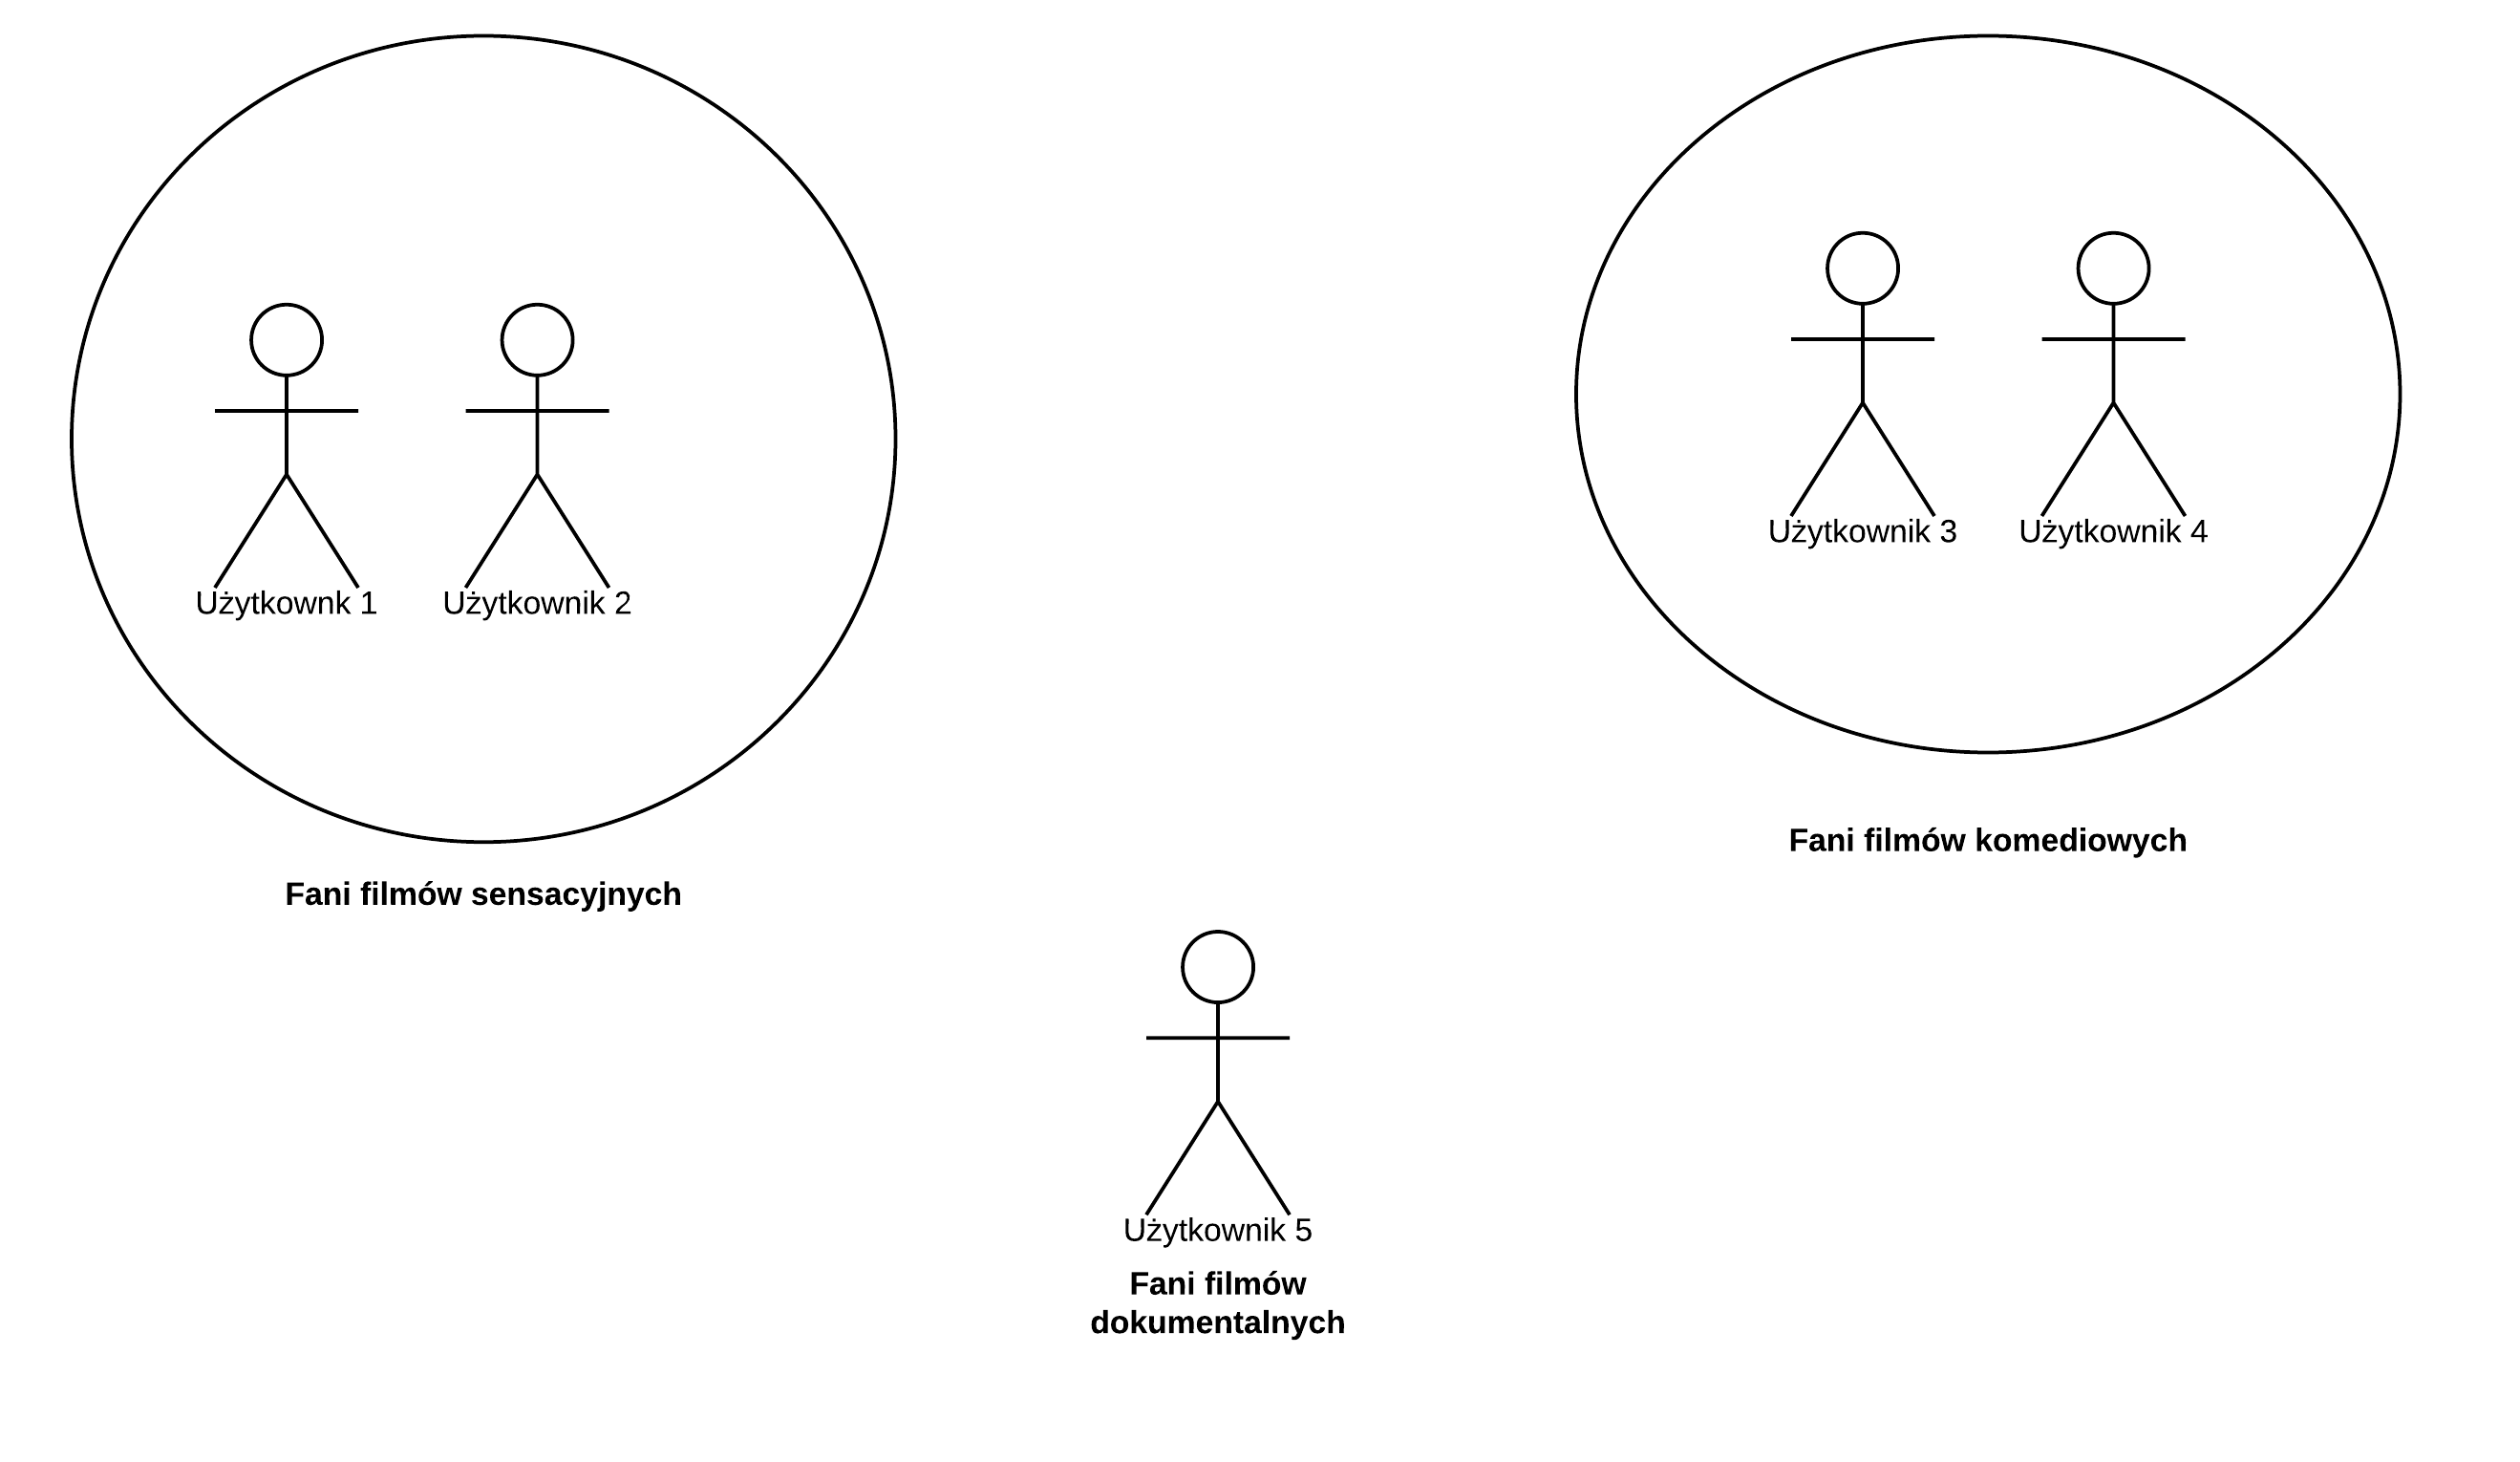
\includegraphics[scale=0.5]{images/grey_sheep.png}
    \caption{Czarna owca - przykład}
    \label{fig:grey-sheep}
\end{figure}

Długi ogon - następuje w momencie, gdy rekomendacja opiera się na produktach podobnych do siebie. Wtedy użytkownicy oglądają tylko część oferowanych przez serwis przedmiotów. Zjawisko to objawia się tym, że produkty, które potencjalnie mogą się podobać konsumentowi nie zostaną mu zaprezentowane. Zjawisko w formie graficznej zaprezentowano na rys. \ref{fig:long-tail} - kolor żółtym zaznaczono długi ogon.

\begin{figure}
    \centering
    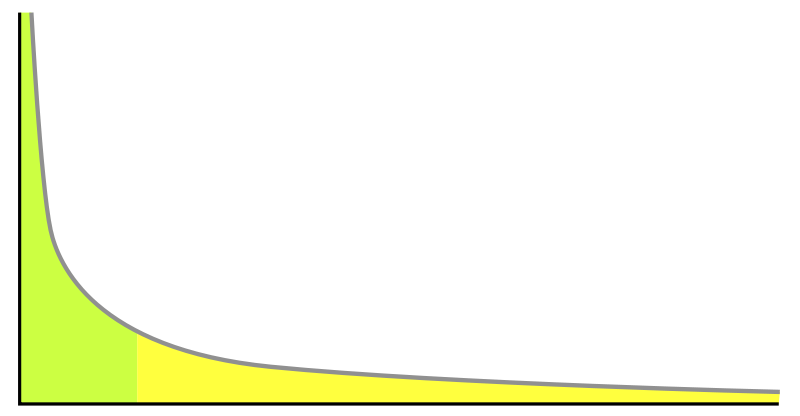
\includegraphics[scale=0.4]{images/long_tail.png}
    \caption{Długi ogon}
    Źródło: Hay Kranen
    \label{fig:long-tail}
\end{figure}

Zimny start (ang \textit{cold-start)} - występuje w momencie rejestracji do systemu nowego użytkownika lub przedmiotu. Przedmioty nie mogą zostać zarekomendowane, ponieważ nie mają żadnej oceny natomiast nowi klienci dokonali zbyt mało ocen.

\section{Content-based filtering}
Podejście bazujące na cechach (ang. \textit{Content-based filtering}) oparte jest na założeniu, że użytkownik polubi przedmioty o podobnej charakterystyce do tych, które poprzednio zostały przez niego polubione (schemat działania przedstawiony na rys. \ref{fig:content-based}). Do tego celu wykorzystywane są opisy produktów (na przykład przedstawione w formie tagów) do generowania rekomendacji. Plusem tego podejścia jest fakt, że do przeprowadzenia rekomendacji nie są potrzebne dane użytkownika, jednak wymagany jest dokładny opis oraz cechy charakterystyczne danego produktu. Przykładami takich cech może być zawartość książki lub sygnał akustyczny utworu muzycznego.


todo dodać coś

eeee

eeee

eeee

\begin{figure}
    \centering
    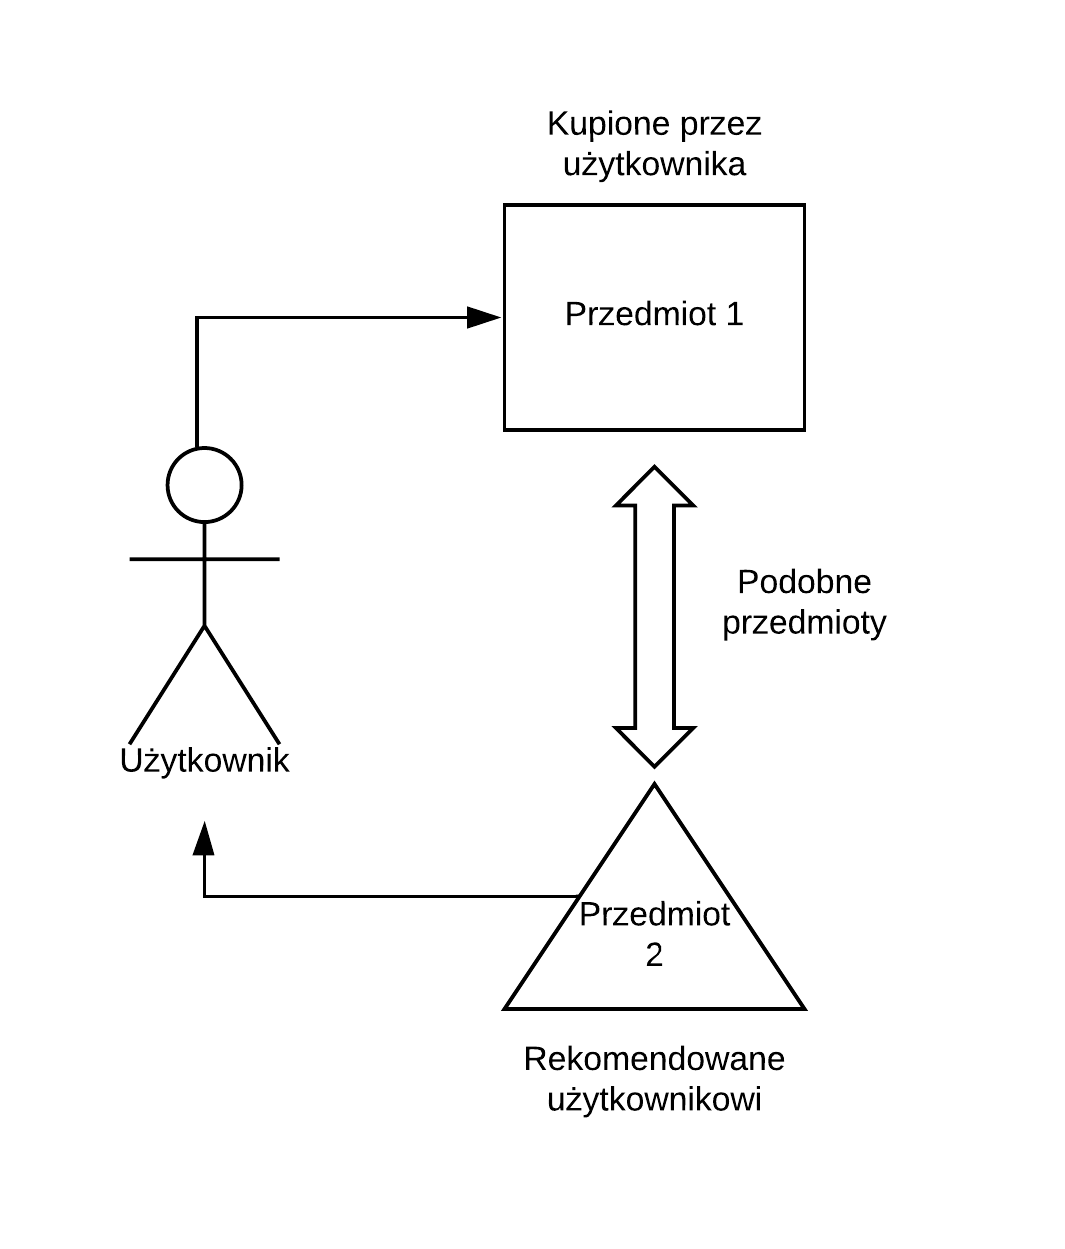
\includegraphics[scale=0.7]{images/content-based.png}
    \caption{Sposób działania mechanizmu \textit{Content-based filtering}.}
    Źródło: opracowanie własne na podstawie \cite{challenges_solutions_survey}
    \label{fig:content-based}
\end{figure}

\section{Collaborative filtering}

Podejście to nie wykorzystuje cech charakterystycznych przedmiotu (tak jak to było w metodzie \textit{Content-based filtering}), jednak problemem jest wygenerowanie rekomendacji dla nowego użytkownika lub produktu (\textit{cold start}). Metoda ta stosowana jest w dużych, komercyjnych aplikacjach. Ma wiele dobrze poznanych, różnorodnych algorytmów i wariacji przez co stosowana jest w wielu domenach.

Opisywana metoda może zostać podzielona na dwie podkategorie:

\begin{itemize}
    \item podejście pamięciowe (\textit{ang. memory based}) rekomenduje przedmiot na podstawie zbioru poprzednio ocenionych przez użytkownika przedmiotów. Dla przykładowego użytkownika \textit{u}, predykcja wyliczana jest na podstawie podobnych do niego użytkowników (główna idea przedstawiona na rys. \ref{fig:collaborative}) lub przedmiotów podobnych do tych, które wcześniej ocenił. Miara podobieństwa najczęściej obliczana jest korelacją Pearsona, wyjaśnioną dalej, lub podobieństwem kosinusowym, które jest iloczyn skalarnym dwóch wektorów, i reprezentuje kosinus kąta pomiędzy dwoma wektorami reprezentującymi przedmiotu. Dwa dokumenty są identyczne, wtedy gdy wartość miary wynosi 1. Natomiast wartość 0 oznacza, że dokumenty są do siebie niepodobne,
    
\begin{figure}[H]
    \centering
    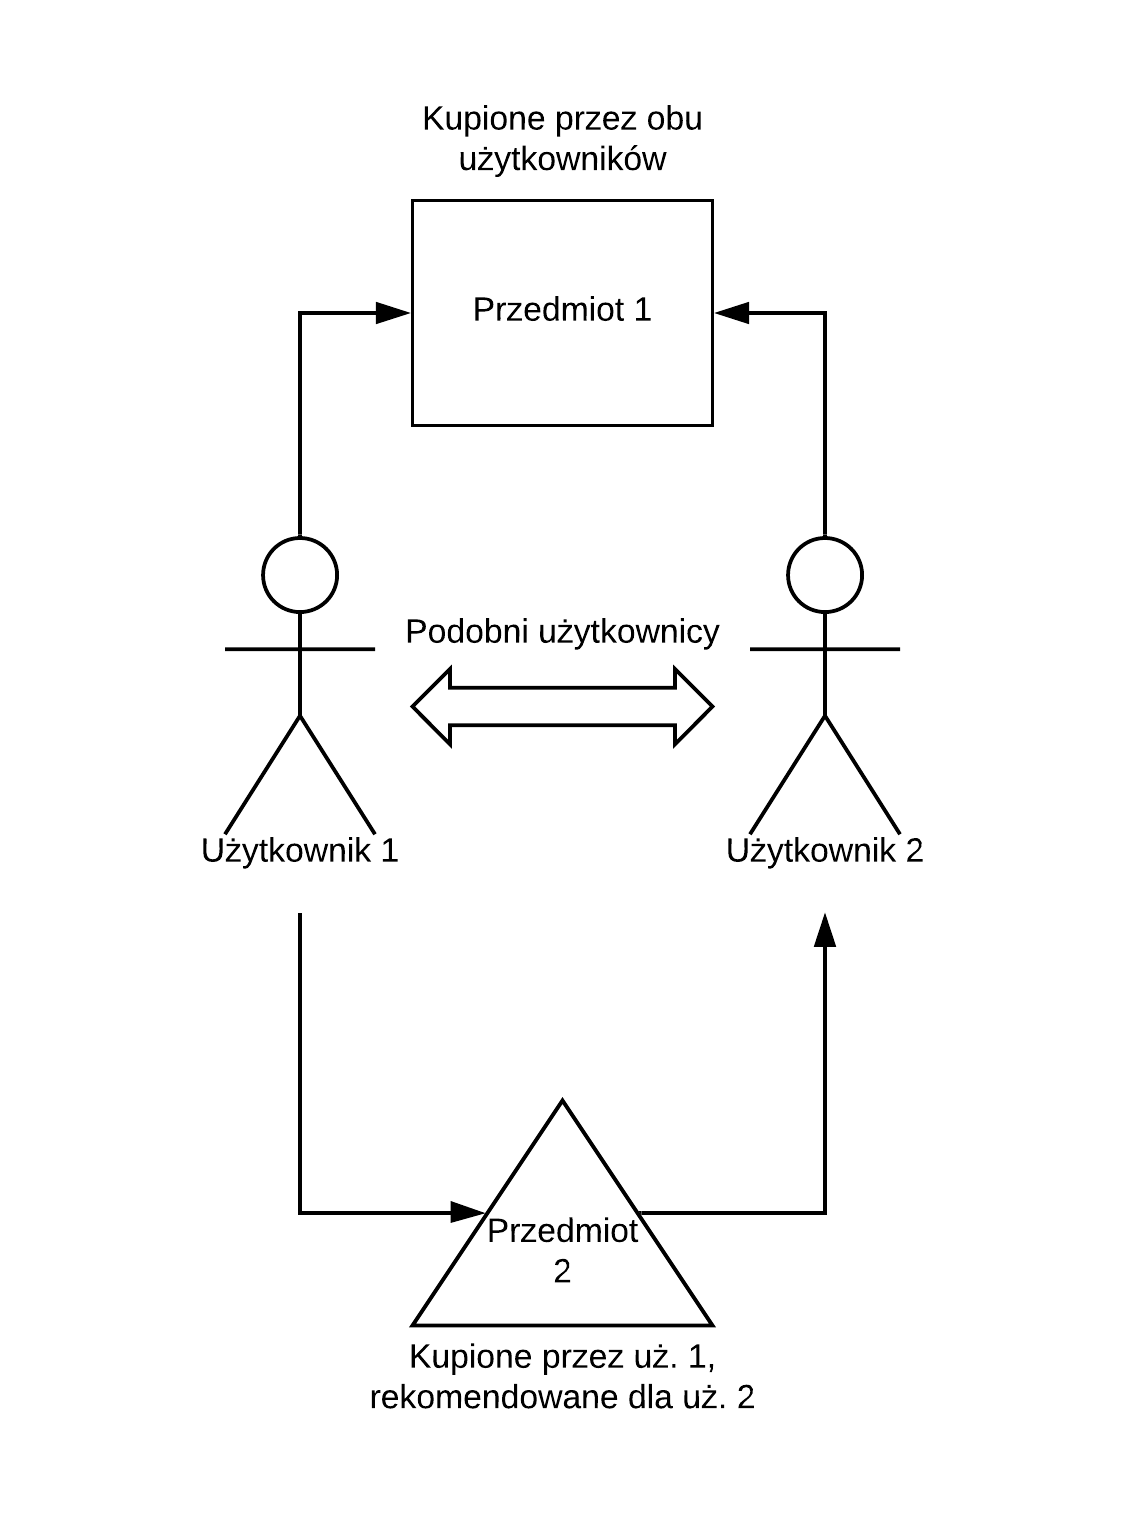
\includegraphics[scale=0.6]{images/collaborative.png}
    \caption{Sposób działania mechanizmu \textit{Collaborative filtering}.}
    Źródło: opracowanie własne na podstawie \cite{challenges_solutions_survey}
    \label{fig:collaborative}

\end{figure}
    \item podejście modelowe (\textit{ang. content based}) wykorzystuje dane historyczne. Jedną z najczęściej stosowanych metod w tym podejściu jest faktoryzacja macierzy, która zakłada, że użytkownicy oceniają przedmioty na podstawie pewnych cech. W przypadku muzyki może to być jej gatunek lub wykonawca. W takim przypadku system rekomendacyjny jest w stanie odkryć czynniki umożliwiające lepszą skuteczność systemu (liczba czynników powinna być mniejsza od liczby użytkowników i przedmiotów). 
\end{itemize}

W celu określenia miary podobieństwa pomiędzy użytkownikami najczęściej stosowana jest korelacja Pearsona. Definiowana jest ona w następujący sposób:

\begin{equation}
Pearson(x,y) = \frac{\sum\limits_{i=1}^n(x_i - \overline{x})(y_i - \overline{y})}{\sqrt{\sum\limits_{i=1}^n(x_i - \overline{x})^2}\sqrt{\sum\limits_{i=1}^n(y_i - \overline{y})^2}},
\end{equation}
dla podobieństwa dwóch użytkowników wzór wygląda następująco:

\begin{equation}
Pearson(a,b) = \frac{\sum\limits_{p \in P}(r_{a,p} - \overline{r}_a)(r_{b,p} - \overline{r}_b)}{\sqrt{\sum\limits_{p \in P}(r_{a,p} - \overline{r}_a)^2}\sqrt{\sum\limits_{p \in P}(r_{b,p} - \overline{r}_b)^2}},
\end{equation} gdzie:
\begin{itemize}
    \item a,b -- użytkownicy,
    \item $r_{a,p}$ -- ocena użytkownika a dla przedmiotu p,
    \item $r_{b,p}$ -- ocena użytkownika b dla przedmiotu p,
    \item $\overline{r}_a$ -- średnia ocen użytkownika a,
    \item $\overline{r}_b$ -- średnia ocen użytkownika b,
    \item P -- zbiór przedmiotów ocenionych przez obu użytkowników.
\end{itemize}

Uzyskane w ten sposób wartości są z przedziału [-1; 1], im wyższa liczba tym użytkownicy są do siebie bardziej podobni.

\section{Knowledge-based filtering}

Podejście oparte o wiedzę polega na wykorzystaniu źródeł wiedzy, które nie zostały uzyskane za pomocą poprzednio omawianych metod. Rekomendacje generowane są na podstawie wiedzy dziedzinowej preferencji użytkownika, cech przedmiotów oraz jak te cechy mogą spełniać potrzeby użytkownika. Wyróżnia się dwa podejścia:
\begin{itemize}
    \item oparte o przypadek (ang. \textit{case-based}) - używają  metryk podobieństwa do uzyskania przedmiotów zgodnych z potrzebami użytkownika,
    \item oparte o ograniczenia (ang. \textit{constraint-based}) - opiera działanie na zbiorze reguł, aby znaleźć przedmioty spełniające wymagania użytkowników.

\end{itemize}

Oba podejścia wymagają od użytkownika podania wymagań, na podstawie których system będzie próbował otrzymać odpowiedź na żądanie użytkownika.

\section{Podejście hybyrdowe}

Podejście hybrydowe ma na celu zniwelować wady pojedynczych metod poprzez połączenie dwóch lub więcej mechanizmów. Najczęściej stosowaną kombinacją jest \textit{Content-based} wraz z \textit{Collaborative filtering}. 

Koncepcja \textit{Content-Boosted Collaborative Filtering} wykorzystuje pseudowektor ocen użytkowników $V_{u}$, który zawiera oceny użytkownika $u$ oraz predykcję ocen przedmiotów nieocenionych przez niego. 

\begin{equation}
V_{u,i} = \left\{ \begin{array}{ll}
\textrm{$r_{u,i}$ :} & \textrm{gdy użytkownik u ocenił przedmiot i}\\
\textrm{$c_{u,i}$ :} & \textrm{w przeciwnym przypadku}
\end{array} \right.
\end{equation} gdzie:
\begin{itemize}
    \item $r_{u,i}$ - ocena podana przez użytkownika u,
    \item $r_{u,i}$ - przewidywana ocena przez czysty system typu \textit{content-based}. 
\end{itemize}
Tak utworzone pseudowektory dla wszystkich użytkowników tworzą macierz V, na której zostanie przeprowadzone filtrowanie kolaboracyjne.

\section{Sposoby ewaluacji}\label{metryki}

Ważnym aspektem podczas tworzenia systemów rekomendacyjnych jest ocena działania zaimplementowanego algorytmu. Ze względu na środowisko można je podzielić na testy offline oraz online lub na statystyczne (np. MAE) i wspierające decyzje (np. AUC) \cite{herlocker}. Ewaluacja offline jest najprostszym podejściem, ponieważ nie wymaga interakcji z rzeczywistym odbiorcą systemu. Natomiast drugie podejście daje lepsze rezultaty jednak wymaga to dużych nakładów finansowych oraz w niektórych przypadkach ciężko zrozumieć powiązania pomiędzy użytkownikami a właściwościami systemu. Podstawowymi miarami dla systemu działającego na produkcji to na przykład współczynnik klikalności (ang. \textit{click through rate} - CTR) oraz sumaryczna wartość transakcji (ang. \textit{gross merchandise volume} - GMV). Ponadto stosuje się testy na małej liczbie użytkowników w kontrolowanym środowisku oraz raportowanie ich doświadczeń podczas pracy z systemem.

Zbiór danych dzielony jest na treningowy, walidacyjny oraz testowy. Zbiór treningowy wykorzystywany jest podczas uczenia modelu, natomiast zbiór walidacyjny do sprawdzenia skuteczności wyuczonego modelu. Po uzyskaniu zadowalających wyników wykorzystuje się zestaw testowy do wyliczenia skuteczności modelu. Jakość predykcji w systemach rekomendacyjnych mierzona jest poprzez następujące miary:

Średni błąd kwadratowy (\textit{ang. Mean Absolute Error}) - mierzy bezwzględny błąd pomiędzy wyestymowaną wartością, a prawdziwą.

\begin{equation}
    MAE = \frac{\sum\limits_{i}^{N}|\hat{r}_{u,i} - r_{u,i}|}{N},
\end{equation} gdzie:
\begin{itemize}
    \item $\hat{r}_{u,i}$ - predykcja oceny użytkownika u dla przedmiotu i,
    \item $r_{u,i}$ - rzeczywista ocena,
    \item N - liczba wszystkich ocen w danych testowych.
\end{itemize}

Pierwiastek średniego błędu kwadratowego (\textit{ang. Root Mean Square Error}) - wzmacnia błąd średniokwadratowy pomiędzy przewidywaną wartością, a rzeczywistą. Sprawdza się, gdy błąd ma duży wpływ na decyzje użytkowników.

\begin{equation}
    RMSE = \sqrt{\frac{\sum\limits_{i}^{N}(\hat{r}_{u,i} - r_{u,i})^2}{N}},
\end{equation}

Precyzja (ang. \textit{Precision}) jest to stosunek prawidłowo sklasyfikowanych elementów do wszystkich otrzymanych.

\begin{equation}
    Precision = \frac{T_p}{T_p + F_p},
\end{equation} \\
Czułość (ang. \textit{Recall}) jest to stosunek prawidłowo sklasyfikowanych elementów do wszystkich, które powinny zostać rozpoznane.
\begin{equation}
    Recall = \frac{T_p}{T_p + F_n},
\end{equation} \\

\begin{table}[h]
\centering
\caption{Macierz błędów.}
\begin{tabular}{cc|p{2cm}|p{2cm}|}
  \cline{3-4}
  & & \multicolumn{2}{ |c| }{Klasa rzeczywista}
  \\
  \cline{3-4}
  & & pozytywna & negatywna \\ \cline{1-4}
  \multicolumn{1}{ |c  }{\multirow{2}{*}{Klasa predykowana} } & \multicolumn{1}{ |c| }{pozytywna} & prawdziwie pozytywna ($T_p$) & fałszywie pozytywna ($F_p$)     \\ \cline{2-4}
  \multicolumn{1}{ |c  }{}                        &
  \multicolumn{1}{ |c| }{fałszywa} & fałszywie negatywna ($F_n$) & prawdziwie negatywna ($T_n$)     \\ \cline{1-4}
    \label{macierzBledow}
\end{tabular} 
\end{table}

F1 - średnia harmoniczna dla wartości precyzji i czułośći. 

\begin{equation}
    F1 = \frac{2 * precision * recall}{precision + recall},
\end{equation}

Pole pod krzywą ROC (\textit{ang. Receiver operating Characteristic}) - krzywa ROC pokazuje wydajność klasyfikatora binarnego na dwuwymiarowej płaszczyźnie. Pole pod krzywą ROC jest wykorzystywane do mierzenia zdolności systemu do odróżniania dobrych predykcji od złych. Większa wartość tej metryki oznacza lepszą wydajność systemu. Macierz błędów została przedstawiona w tabeli \ref{macierzBledow}.

\section{Skuteczność metod}

Każda z omówionych we wcześniejszych rozdziałach metod posiada zalety i wady przez co nie zawsze sprawdzają się w danych zastosowaniach. Użycie danej metody musi zostać oparte na rodzaju danych, wielkości systemu oraz domeny w jakiej ma być wykorzystywana. Tabela \ref{tabelaMetProblem} przedstawia poszczególne mechanizmy rekomendacji wraz z odpornością na dany problem, gdzie "-" oznacza podatność, a "+" niewrażliwość.

Mechanizm \textit{content-based} posiada dwie główne zalety. Pierwsza z nich to fakt, że nie jest wymagana żadna wiedza na temat innych użytkowników w momencie, gdy rekomendacje są generowane wyłącznie do jednego, określonego użytkownika. Przez co umożliwia na łatwiejsze skalowanie aplikacji w przypadku wystąpienia znacznego wzrostu liczby użytkowników. Także zastosowanie tego podejścia umożliwia na wychwycenie specyficznych zainteresowań użytkownika przez co rekomendacja obejmuje niszowe obiekty, które podobają się jedynie garstce użytkowników. Jednak wykorzystanie tej techniki wymaga sporej wiedzy dziedzinowej (model może być wyłącznie tak dobry jak wybrane cechy brane pod uwagę przy nauce modelu). Podawane rekomendacje ograniczają się wyłącznie do aktualnych zainteresowań użytkownika (nie są proponowane przedmioty wychodzące poza gust użytkownika).

Systemy rekomendacyjne wykorzystujące podejście \textit{collaborative-filtering} uzyskują zadowalające wyniki związane z wydajnością, jednak nie są odporne na problem zimnego startu. Także problemem może okazać się rzadkość danych, jeżeli wartość wynosi około 0.5 lub więcej wtedy należy rozważyć użycie innego rozwiązania. Wraz ze wzrostem liczby użytkowników rośnie krytycznie problem związany ze skalowalnością takiego systemu (rozmiar macierzy zwiększa się znacząco z napływem nowych użytkowników lub przedmiotów). Oprócz wspomnianych wad zastosowanie tego podejścia nie jest wymaga wiedzy domenowej, ponieważ w celu wytrenowania potrzebna jest wyłącznie macierz sprzężenia zwrotnego. Także wykorzystanie tego modelu umożliwia na pokazanie użytkownikom nowego przedmiotu/obiektu, który podobał się innym podobnym użytkownikom.

Systemy wykorzystujące mechanizm \textit{knowlegde-based} cechują się łatwością w implementacji tak zwanych reguł biznesowych, co w pozostałych rozwiązaniach nie jest tak proste. Metoda nie wymaga wkładu użytkownika do rozpoczęcia działania, przez co nie występuje problem związany z zimnym startem. Jednak zbudowanie systemu opartego na tym mechanizmie jest bardzo drogie, ponieważ wymaga trafnej wiedzy eksperckiej. W aktualnych rozwiązaniach stosowany jest niesamodzielnie, lecz w połączeniu z innymi mechanizmami.  \cite{reviewCurrentRS}

Wydajność, a także zalety i wady związane z podejściem hybrydowym zależy od kombinacji mechanizmów, które zostały użyte do jego stworzenia. Połączenie niektórych metod może spowodować zniwelowanie problemów występujących podczas rekomendowania produktów dla użytkowników.

\begin{table}[h]
\centering
\caption{Odporność mechanizmów rekomendacyjnych na potencjalne problemy.}
\begin{tabular}{|c|c|c|c|c|c|}
\hline
&
\specialcell{Rzadkość\\danych} &
Skalowalność &
\specialcell{Czarna\\owca} &
\specialcell{Długi\\ogon} &
\specialcell{Zimny\\start}
\\
\hline
  
Content-based &
+ &
+ &
+ &
- &
-
\\
\hline
  
Collaborative &
- &
- &
- &
- &
-
\\
\hline

Knowledge-based &
+ &
+ &
+ &
+ &
+
\\
\hline

\specialcell{Podejście\\hybyrdowe} &
+/- &
+/- &
+/- &
+/- &
+/-
\\
\hline
\end{tabular} 
\label{tabelaMetProblem}
\end{table}


\chapter{Aspekt bezpieczeństwa w systemach rekomendacyjnych}
Systemy rekomendacyjne muszą gromadzić wiele danych o użytkownikach w celu wykonania trafnego przewidywania potencjalnych obiektów zainteresowania. W zależności od metody serwis dokonuje porównania  profili użytkowników, oblicza podobieństwo pomiędzy użytkownikami czy grupuje użytkowników o zbliżonych cechach. Gromadzone w tym celu dane mogą pozwolić na identyfikacje użytkownika przez co twórcy systemu muszą wybierać pomiędzy prywatnością użytkowników, a skutecznością w dokonywaniu rekomendacji. Taki system z wrażliwymi danymi użytkowników może stać się celem grup hakerskich chcących pozyskać tak cenne informacje. Stąd zapewnienie bezpieczeństwa podczas przesyłania danych pomiędzy serwisami oraz dokonywania obliczeń na nich powinno stać się priorytetem. Jednak większość prac skupia się na zwiększeniu skuteczności czy wydajności \cite{recent_developments}.

\section{Prywatność}
Prywatność w kontekście systemów rekomendacyjnych oznacza, że podczas pracy systemy żadne dane nie mogą wyciec, a także otrzymana predykcja nie powinna pozwolić na identyfikację użytkownika. Na rysunku \ref{fig:podatnosci} przedstawiono potencjalne miejsca, w których dane mogą zostać przechwycone. Jak widać atakujący mogą uzyskać dane podczas wprowadzania ich do systemu, przesyłania ich pomiędzy poszczególnymi komponentami usługi, jak i w trakcie wysłania predykcji do użytkownika. Idealny, zachowujący prywatność system rekomendacyjny powinien być bezpieczny bez znaczącej utraty na wydajności jako całości, a przede wszystkim bez zmniejszenia trafności rekomendacji. 
    Y = X + C, gdzie C jest szumem dodanym do oryginalnej macierzy X. W praktyce każdy wiersz C generowany jest niezależnie,
\begin{itemize}
    \item perturbacja danych (ang. \textit{data perturbation}),
    \item bezpieczne obliczanie wieloczęściowe (ang. \textit{secure multiparty computation}).
\end{itemize}

\begin{figure}
    \centering
    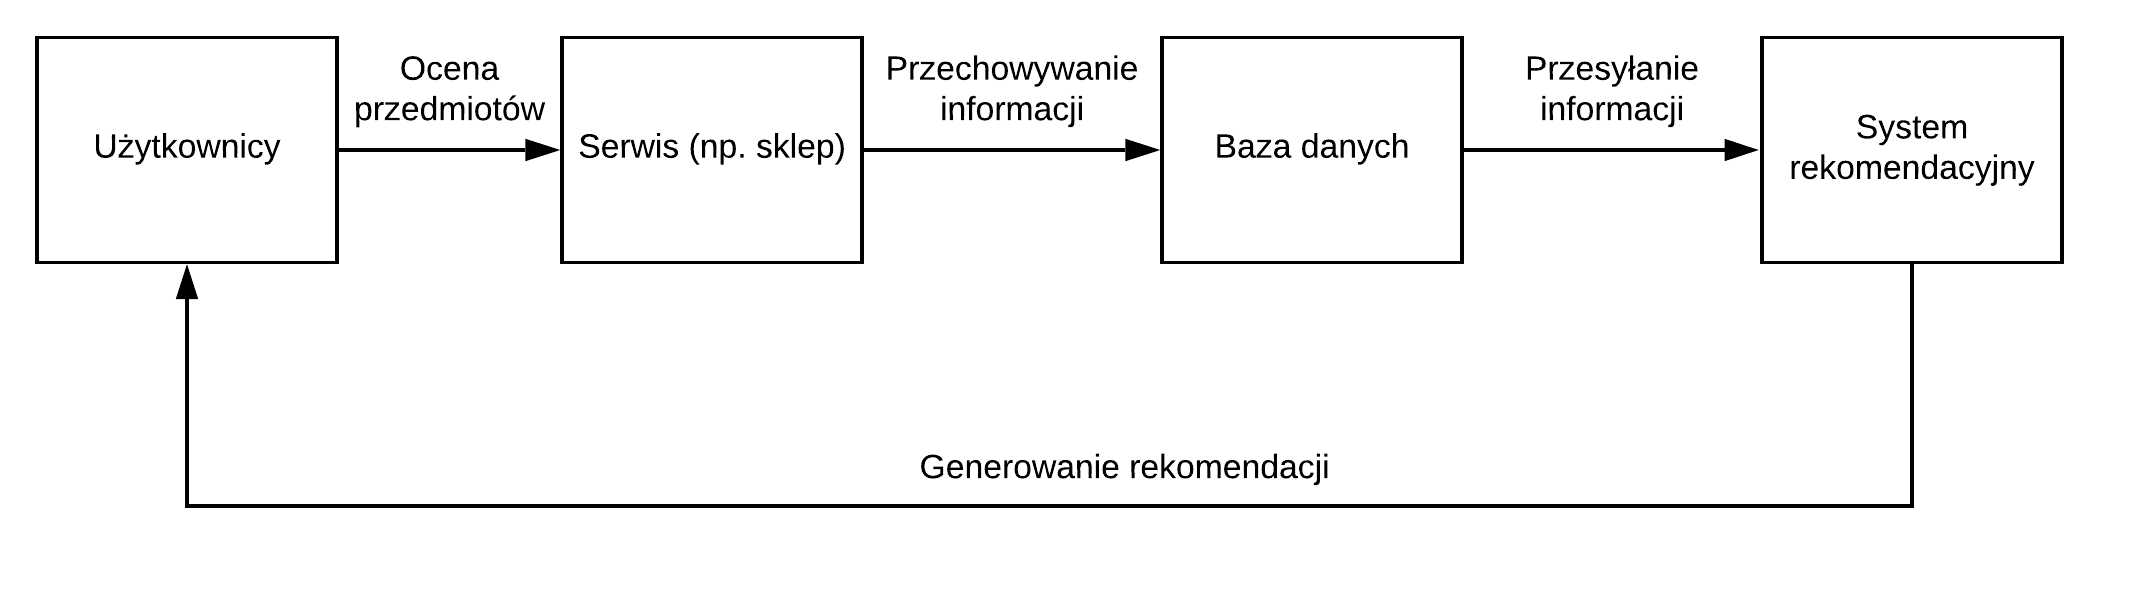
\includegraphics[scale=0.85]{images/podatnosci.png}
    \caption{Potencjalne podatności systemu.}    Źródło: opracowanie własne na podstawie \cite{practicalPrivacy}

    \label{fig:podatnosci}
\end{figure}
\section{Perturbacja danych}
Właściciel danych (użytkownik) dokonuje perturbacji własnych danych, a następnie przesyła je w celu dalszego przetwarzania.
Wyróżniamy następujące rodzaje perturbacji danych:
\begin{itemize}
    \item addytywne - opisane następującym wzorem 
    Y = X + C, gdzie C jest szumem dodanym do oryginalnej macierzy X. W praktyce każdy wiersz C generowany jest niezależnie,
    \item multiplikatywne - opisane wzorem Y = MX, gdzie M jest to macierz przez którą przekształcana są dane źródłowe. W przypadku tej metody nie ma gwarancji, że zostanie zachowana prywatność (przypadek w którym atakujący zna porcję danych w zbiorze X oraz ich odpowiednik w zbiorze M),
    \item prywatność różnicowa - wyróżnia się trzy podejścia w zależności od momentu wprowadzenia szumu: do danych wejściowych, w trakcie przetwarzania lub do danych wyjściowych.
\end{itemize}

Głównym problemem w wykorzystaniu perturbacji danych w celu zapewnienia prywatności jest brak gwarancji, że uzyskane wyniki będą tak samo trafne jak w przypadku bez wprowadzenia szumu w danych.

\section{Bezpieczne obliczanie wieloczęściowe}

Metoda pozwala rozproszonym stronom na wspólne obliczanie bez konieczności odkrywania ich prywatnych danych wejściowych oraz wyjściowych. Ponadto zastosowania obliczania wieloczęściowego nie wymaga użycia zaufanej trzeciej strony (bezpieczeństwo pozostaje takie samo jak w przypadku wykorzystania trzeciej strony). 
Wyróżniane są następujące rozwiązania:
\begin{itemize}
    \item rozwiązania oparte na bezpiecznym dodawaniu wektorów (\textit{ang. Secure Vector Addition based Solutions}),
    \item szyfrowanie homomorficzne,
    \item podejścia oparte na bezpiecznych produktach skalarnych (\textit{ang. Secure scalar product based approach}),
    \item podejścia oparte o "zniekształcony obwód" (\textit{ang. Garbled circuit based approach}).
\end{itemize}

Jednak bezpieczne obliczanie wieloczęściowe nie sprawdza się w komercyjnych rozwiązaniach opartych o rekomendacje. Spowodowane jest tym, że metoda ta na ten moment nie może być rozpatrywana przy systemach wymagających działania w czasie rzeczywistym. \cite{secureMultipartyComputation}


\chapter{Model systemu rekomendacyjnego chroniącego prywatność}

W rozdziale zaproponowanie rozwiązania zwiększającego bezpieczeństwo oraz zachowanie prywatnych danych użytkownika. W tym celu wykorzystano \textit{Federated learning} omówiony w rozdziale \ref{section:federatedLearning} wraz z dodatkowymi zabezpieczeniami mającymi na celu zniwelować przedstawione problemy związane z tym rozwiązaniem. Także przedstawiono jak mógłby wyglądać proces przygotowania takiej metody dla nowo-powstałego systemu jak i dla już zaimplementowanego systemu z wykorzystaniem dostępnych bibliotek i technologii.

\section{Projekt rozwiązania}

W proponowanym rozwiązaniu wyróżniono trzech aktorów. Pierwszy z nich, zwykły użytkownik uczestniczy w normalnym przebiegu zaproponowanym w rozwiązaniu \textit{Federated learning}. Użytkownik na podstawie swoich danych poprawia otrzymany przez serwer model, następnie bez ujawniania swoich danych przekazuje dalej wyłącznie poprawiony przez siebie model.

Jednym z potencjalnych problemów może być założenie, że użytkownicy będą uczciwie uczestniczyć w całym omawianym procesie. Oznacza, to że użytkownik może zmniejszyć skuteczność modelu rekomendacji poprzez umieszczenie w nich niepoprawnych danych (niezgodnych z rzeczywistością). W przypadku pojedynczego użytkownika, który próbuje zakłócić pracę systemu istnieje mechanizm uśredniający otrzymane wyniki od wszystkich użytkowników. Jednak w przypadku zorganizowanego ataku z wielu kont wyłącznie normalizacja może nie być wystarczająca. W celu poradzenia sobie z tym problemem wprowadzono drugi typ aktora - użytkownik niezaufany, który ma możliwość wyłącznie otrzymania modelu od serwera głównego. Jest on wyłączony z usprawnienia udostępnianego modelu (nie wysyła on swoich rezultatów uczenia). Tego typu użytkownik po określonym czasie użytkowania systemu, ilości wystawionych ocen lub po odpowiednim procesie weryfikacyjnym może zostać przemianowany na zwykłego użytkownika uczestniczącego w procesie usprawniania wspólnego modelu.

Kolejnym problemem może być koszt nauki na systemach mobilnych. Niektórzy użytkownicy mogą posiadać słabszy sprzęt (zasoby sprzętowe czy bateria), który może uniemożliwić ponowne uczenie otrzymanego modelu na urządzeniu. W przypadku wolnego łącza lub jego braku, problemem może być pobieranie lub odesłanie modelu do głównego serwera. W tym celu użytkownik z ograniczonymi zasobami zostałby zmuszony do przesłania swoich zaszyfrowanych danych do serwera, tam wykorzystując właściwości szyfrowania homomorficznego model zostałby zaktualizowany, a rekomendacje przesłane do użytkownika.

\section{Fazy budowania systemu rekomendacyjnego}

Podczas implementacji systemu rekomendacyjnego wykorzystano typowy przepływ (przedstawiony na rysunku \ref{fig:rs_pipeline}) używany do tworzenia tego typu serwisów, który składa się z następujące pięć faz \cite{rs_in_real}:
\begin{itemize}
    \item wstępne przetwarzanie - na ten etap składają się czynności związane z transformacją danych do macierzy użytkownik-produkt oraz normalizacja w celu spłaszczenia wartości odstających (użytkownicy, którzy są nad wyraz pozytywni oraz negatywni w stosunku do dawania ocen),
    \item trenowanie - proces budowania modelu,
    \item optymalizacja hiper parametrów - wielokrotne trenowanie w celu dostrojenia parametrów w taki sposób, aby uzyskać jak najlepsze wyniki,
    \item przetwarzanie końcowe - sortowanie danych w celu uzyskania N najlepszych rekomendacji dla użytkownika, filtrowanie oraz wykluczenie wcześniej zakupionych lub negatywnie ocenionych przedmiotów,
    \item ewaluacja - testowanie stworzonego modelu poprzez ukrywanie/maskowanie ocen, a następnie użycie miar do ewaluacji (szczegółowo opisane w podrozdziale \ref{metryki}).
\end{itemize}{}

\begin{figure}
    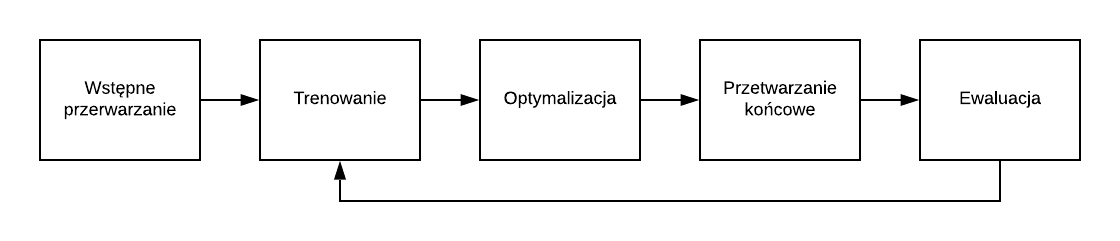
\includegraphics[scale=0.85]{rs_pipeline.png}
    \caption{Fazy przepływu podczas tworzenia systemu rekomendacyjnego.}
    \label{fig:rs_pipeline}
\end{figure}

\section{Dane testowe}

\section{Przegląd dostępnych technologii}

Istnieje wiele dostępnych bibliotek czy frameworków umożliwiające na implementacje rozwiązań typu \textit{Federated learning}. Większość z nich umożliwia na napisanie kodu w języku Python. Jednymi z bardziej popularnych oraz dobrze udokumentowanych są następujące technologie:

\begin{itemize}
    \item PySyft - narzędzie opracowane przez grupę OpenMinded. PySyft rozszerza popularne biblioteki takie jak: PyTorch, Tensorflow oraz Keras o możliwość zdalnego wykonywania, szyfrowania homomorficznego czy obliczenia z wykorzystaniem wielu użytkowników,
    \item Tensorflow Federated - biblioteka wykorzystywana do uczenia maszynowego i innych obliczeń na danych nie scentralizowanych oparta o otwarty kod źródłowy. Stworzona w celu badań oraz eksperymentowania z koncepcją \textit{Federated learning}.
\end{itemize}

\section{Fragmenty implementacji}


\chapter{Podsumowanie}



\medskip

\bibliographystyle{plamsplain}
\bibliography{bibliography}

\end{document}
